\textbf{COLUNI 2022 -- Questão 33}\par\medskip Leia o texto a seguir.

\par

\textbf{Índice global da Fome}

\par

A \textit{Welthungerhilfe} é uma organização de ajuda humanitária que desenvolve trabalhos contra a fome em todo o mundo. Essa organização produz um dos principais relatórios internacionais, com capacidade de abranger os diversos aspectos do fenômeno fome no mundo. O Índice Global da Fome (\textit{Global Hunger Index, GHI}) para o ano de 2020 é representado na ilustração a seguir:

\par

\textbf{ÍNDICE GLOBAL DA FOME 2020}

% COLUNI-AUTO-FIGURES-BEGIN
\begin{figure}[htbp]
\centering
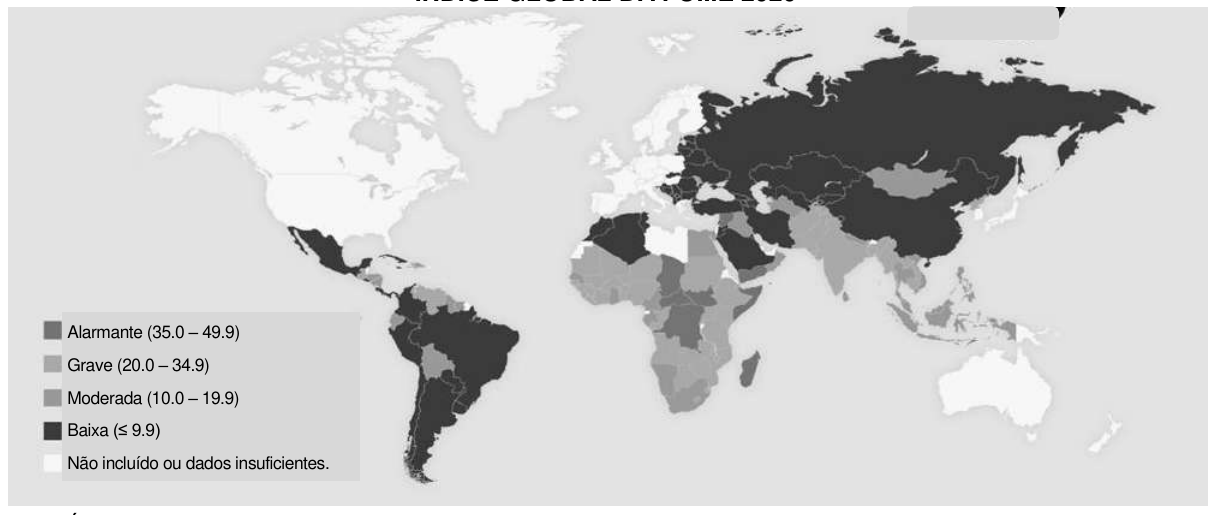
\includegraphics[width=0.95\linewidth]{static/simulados/coluni/figuras/2022/questao-33/figura-1.png}
\end{figure}
% COLUNI-AUTO-FIGURES-END

Fonte: Índice global da fome 2020: uma década até “fome zero” ligando a saúde aos sistemas alimentares sustentáveis. Disponível em: https://www.globalhungerindex.org/pdf/pt/2020.pdf. Acesso em: 12 mar. 2021. pp. 20-21 – (Adaptado).

\par

Após ler o texto e analisar a ilustração sobre O Índice Global da Fome, em relação aos aspectos causadores do fenômeno fome no mundo em 2020, é CORRETO afirmar que:


\begin{enumerate}
\item a crise sanitária, econômica e ambiental provocada pela pandemia da Covid-19 atingiu, de forma
        igualitária, as diferentes regiões do globo.
\item os sistemas alimentares do mundo tornam-se cada vez mais interligados, o que garante a soberania
        alimentar dos países.
\item a incerteza em relação à posse da terra e aos recursos hídricos afeta a segurança alimentar de vários
        países.
\item as políticas globais de doação de alimentos e de solidariedade têm provocado o fim da fome nas diversas
        regiões do mundo.\end{enumerate}
